%\documentclass[]{algotel}
%\usepackage[utf8]{inputenc}
\documentclass[10pt, conference, letterpaper]{IEEEtran}
%
\usepackage[utf8]{inputenc}
\usepackage[english]{babel}
\usepackage{caption}
\usepackage{authblk}
\usepackage{graphicx}

\usepackage{xspace}
\usepackage{graphics} 
\usepackage{mathtools, bm}

\usepackage{amssymb, bm}
\usepackage{complexity}
\usepackage{amsmath,amsthm}

\usepackage{color}
\usepackage{amsmath}
%\usepackage[colorlinks=true,breaklinks=true,linkcolor=blue]{hyperref}
\captionsetup{justification=centering,margin=0.5cm}


\newcommand\pall{\textsc{pall}\xspace}
\newcommand{\todo}[1]{{\color{red} TODO: {#1}}}	
\newtheorem{prop}{Proposition}

\newtheorem{theorem}{Theorem}
\newtheorem{corollary}{Corollary}

\renewcommand{\thefootnote}{\*}

\graphicspath{{img/}}
\title{Deterministic contention management for low latency Cloud RAN over an optical ring}
\makeatletter
\renewcommand*{\thetable}{\arabic{table}}
\renewcommand*{\thefigure}{\arabic{figure}}
\let\c@table\c@figure
\makeatother 

\author[1]{Dominique Barth}
\author[1,2]{Ma\"el Guiraud}
\author[1]{Yann Strozecki}
\affil[1]{David Laboratory, UVSQ}
\affil[2]{Nokia Bell Labs France}

\begin{document}

\maketitle


\begin{abstract}
The N-GREEN project has for goal to design a low cost optical ring technology with good performances (throughput, latency$\dots$) without using expensive end-to-end connections. We study the compatibility of such a technology with the development of the Cloud RAN, a latency critical application which is a major aspect of 5G deployment. We show that deterministically managing Cloud RAN traffic minimizes its latency while also improving the latency of the other traffics. 

\end{abstract}


\section{Introduction}

\footnote{This work was developed around the ANR N-GREEN project. The authors thank the Nokia Bell Labs team for their collaboration.} Telecommunication network providers have to design inexpensive networks supporting an increasing amount of data and online applications. Many of these applications require QoS guarantees, like minimal throughput and/or  maximal latency. The N-GREEN project aims to design a high performing optical ring while ensuring a minimal cost for providers. The current solutions with good QoS~\cite{pizzinat2015things,tayq2017real}, establish end-to-end direct connections (E2DE) between the nodes, which is extremely expensive. The N-GREEN optical ring is designed to ensure good performance for a low cost: the hardware it requires scales linearly with the number of nodes while E2DE scales quadratically making it impractical for more than a few nodes.


In this article, we study a Cloud RAN (C-RAN) application based on the N-GREEN optical ring described in~\cite{ngreenarchitecture,uscumlic2018scalable}. C-RAN is one of the major area of development for 5G; it consists in centralizing or partially centralizing the computation units or {\bf BaseBand Units} (BBU) of the {\bf Remote Radio Heads} (RRH) in one datacenter~\cite{mobile2011c}. Periodically, each RRH on the field sends some uplink traffic to its associated BBU in the datacenter, then, after a computation, the BBU sends the same quantity of downlink traffic back to the RRH. The latency of the messages between the BBU and the RRH is critical since some services need end-to-end latency as low as $1$ms~\cite{3gpp5g,boccardi2014five}.


Nowadays, the traffic is managed by statistical multiplexing~\cite{kern2006applying}. Here, we propose an SDN approach to {\bf deterministically} manage the periodic C-RAN traffic by choosing emission timing. Indeed, Deterministic Networking is one of the main method considered to reduce the E2E latency~\cite{finn-detnet-architecture-08}. In a previous work~\cite{dominique2018deterministic}, the authors have studied a similar problem for a star shaped network. In contrast with our previous work, finding emission timings so that different periodic sources do not use the same resource is easy in the context of the N-GREEN optical ring with a single data-center. However, we deal with two additional difficulties arising from practice: the messages from RRHs are scattered (because of the electronic to optic interface) and there are other traffics whose latency must be preserved. It turns out that the deterministic management of CRAN traffic we propose reduces the latency of CRAN traffic to the physical delay of the routes, while reducing the latency of the other traffics by smoothing the load of the ring over the period. To achieve such a good latency, our solution needs to reserve ressources in advance, which slightly decreases the maximal load the N-GREEN optical ring can handle. Such an approach of reservation of the network for an application (CRAN in our context) relates to network slicing~\cite{jiang2016network} or virtual-circuit-switched connections in optical networks~\cite{cadere2010virtual,szymanski2016ultra}.

In Sec.~\ref{sec:model}, we model the optical ring and the traffic flow. In Sec.~\ref{sec:oportmethods}, we experimentally evaluate the latency when using stochastic multiplexing to manage packet insertions on the ring, with or without priority for C-RAN packets. In Sec.~\ref{sec:deterministicalgorithms}, we propose a deterministic way to manage C-RAN packets without buffers, which guarantees to have zero latency from buffering. We propose several refinements of this deterministic sending scheme to spread the load over time, which improves the latency of best effort packet, or in Sec.~\ref{sec:maxant} to allow the ring to support a maximal number of antennas at the cost of a very small latency for the C-RAN traffic. 

\section{Model of C-RAN traffic over an optical ring}
\label{sec:model}
    
  \paragraph{N-GREEN Optical ring}
   
  The unidirectional optical ring is represented by an oriented cycle. The vertices of the cycle represent the nodes of the ring, where the traffic arrives. The arcs $(u,v)$ of the cycle have an integer weight $\omega(u,v)$ which represents the time to transmit a unit of information from $u$ to $v$. By extension, if $u$ and $v$ are not adjacent, we denote by $\omega(u,v)$ the size of the directed path from $u$ to $v$.  The \textbf{ring size} is the length of the cycle, that is $\omega(u,u)$ and we denote it by $RS$. A {\bf container}, of capacity $C$  expressed in bytes, is a basic unit of data in the optical ring. 
  
  The time is discretized: a unit of time corresponds to the time needed to fill a container with data.
  As shown in Fig.~\ref{fig:containers}, the node $u$ can fill a container with a data packet of size less than $C$ bytes at time $t$ if the container at position $u$ at time $t$ is \emph{free}. 
  If there are several packets in a node or if a node cannot fill a container, because it is not free, 
  the remaining packets are stored in the {\bf insertion buffer} of the node. 
  A container goes from $u$ to $v$ in $\omega(u,v)$ units of time. The ring follows a {\bf broadcast and select scheme with emission release policy}: When a container is filled by some node $u$, it is freed when it comes back at $u$ after going through the whole cycle.
   
  
  \begin{figure}[h!]

        \begin{center}
      \hspace{-2.3cm}\includegraphics[scale=0.65]{containers}
   
  % \vspace{0.5cm}
   
      %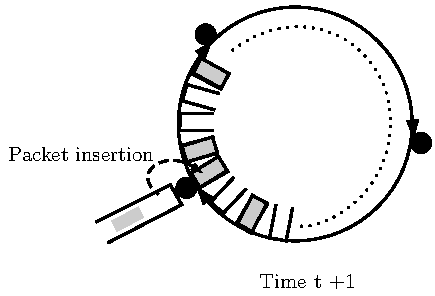
\includegraphics[scale=0.7]{containers2}
      \end{center} 

   
     \caption{Dynamic behavior of the ring.}\label{fig:containers}

  \end{figure}
  
     \paragraph{C-RAN traffic}
   
   The RRHs are the source of the {\bf deterministic and periodic} C-RAN traffic.
   There are $k$ RRHs attached to the ring and several RRHs can be attached to the same vertex. An RRH is linked to a node of the ring through an electronic interface of bit rate $R$ Bps.
   The ring has a larger bit rate of $F\times R$ Bps. The integer $F$ is called the {\bf acceleration factor} between the electronic and the optical domains. A node aggregates the data received on the electronic interface during $F$ units of time to create a packet of size $C$ and then puts it in the insertion buffer.
%   fills a container of the ring with this data. 
  In each period $P$, an RRH emits data during a time called \textbf{emission time} or $ET$. Hence the RRH emits $ET / F$ packets, i.e. a container of size $C$ each $F$ units of time during the emission time, as shown in Fig.~\ref{fig:interface}.
   %Each period $P$, an RRH emits $ET / F$ packets, i.e. a packet of size $C$ each $F$ units of time during a time $ET$ (emission time),
   
   The data of the RRH $i$ arrives at some node $u$ at a time $m_i$ in a period called {\bf offset}. The offsets can be determined by the designer of the system and can be different for each RRH but must remain the same over all periods. We assume that all BBUs are contained in the same data-center attached to the node $v$. The data from $u$ is routed to its BBU at node $v$ through the ring and arrives at time $m_i + \omega(u,v)$ if it has been inserted in the ring upon arrival. Then after some computation time (which w.l.o.g. is supposed to be zero), an answer is sent back from the BBU to the RRH. The same quantity of data is emitted by each BBU or RRH during any period.
   
   The {\bf latency} of a data packet is defined as the time it waits in an insertion buffer.
   Indeed, because of the ring topology, the routes between RRHs and BBUs are fixed, thus we cannot reduce the physical transmission delay of a data which depends only on the size of the arcs used. Moreover, there is only one buffering point in the N-GREEN optical ring, the insertion buffer of the node at which the data arrives. Hence, in this context, to minimize the end-to-end delay, we need to minimize the (logical) latency.
   In particular, we want to reduce the latency of the C-RAN traffic to \textbf{zero}, both for the RRHs (uplink) and the BBUs (downlink). In Sec.~\ref{sec:deterministicalgorithms} we propose a deterministic mechanism with zero latency for C-RAN which also improves the latency of other data going through the optical ring. We shortly describe the nature of this additional traffic in the next subsection.
   
    
\begin{figure}[h!]
\begin{center}   

      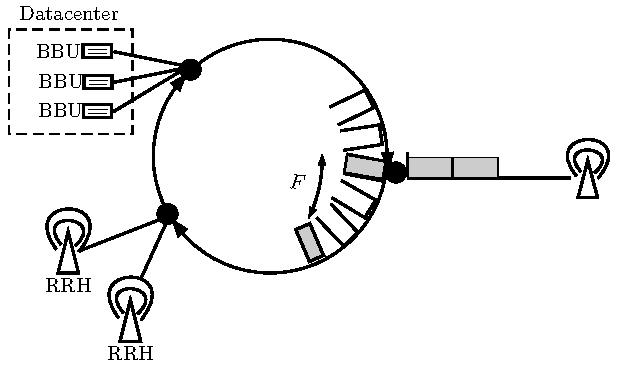
\includegraphics[scale=0.7]{interface.pdf}
     \caption{Insertion in the N-GREEN optical ring.}\label{fig:interface}
     
\end{center}
  \end{figure}


\paragraph{Best effort traffic}

The optical ring supports other traffics, corresponding to the internet flow. We call this traffic \textbf{Best Effort} (BE). We want it to have the best possible distribution of latency, but since BE traffic is less critical than C-RAN traffic, we impose no hard constraint on its latency. At each node of the ring, a {\bf contention buffer} is filled by a batch arrival process of BE data. 
This batch arrival process consists in generating, at each unit of time, a quantity of data drawn from a bimodal distribution to modelize the fact that internet traffic is bursty. Then, according to the fill rate of the contention buffer and the maximum waiting time of the data, a packet of size at most $C$ is created by aggregating data in the contention buffer. This packet is then put in the insertion buffer of the node. Hence, the arrival of BE messages can be modeled by a temporal law that gives the distribution of times between two arrivals of a BE packet in the insertion buffer. The computation of this distribution for the parameters of the contention buffer used in the N-GREEN optical ring is described in~\cite{Cast1810:Performance}. We use this distribution in our experiments to modelize BE packet arrival in the insertion buffer.

   \section{Evaluation of the latency on the N-GREEN optical ring}
   \label{sec:oportmethods}
   
   
  We first study the latency of the C-RAN and BE traffics when the ring follows an opportunistic insertion policy: When a free container goes through a node, it is filled with a packet of its insertion buffer, if there is one.
 Two different methods to manage the insertion buffer are experimentally compared. First, the \textbf{FIFO} rule, that consist in managing the C-RAN and BE packets in the same insertion buffer. Then, when a free container is available, the node fills it with the oldest packet of the insertion buffer, without distinction between C-RAN and BE. This method is compared to a method called \textbf{C-RAN priority} that uses two insertion buffers: one for the BE packets, and another for the C-RAN packets. The C-RAN insertion buffer has the priority and is used to fill containers on the ring while it is non empty before considering the BE insertion buffer.  
 
We compare experimentally these two methods in the simplest topology: The lengths of the arcs between nodes are equal and there is one RRH by node. The experimental parameters are given in Table~\ref{fig:params} and chosen following~\cite{ngreenarchitecture}. In this experiment, the offsets of the RRH have been randomly distributed in the period. The results are computed over $1,000$ experiments (with different random offsets) where the optical ring is simulated during $1,000,000$ units of time. Fig.~\ref{fig:resultopport} gives the cumulative distribution of both C-RAN and BE traffics latencies for the FIFO and the C-RAN priority methods. The source code in C of the experiments can be found on one of the authors' webpage~\cite{webpage}.
   \vspace{0.5cm}
  \hspace{-0.75cm}


        \begin{center}
      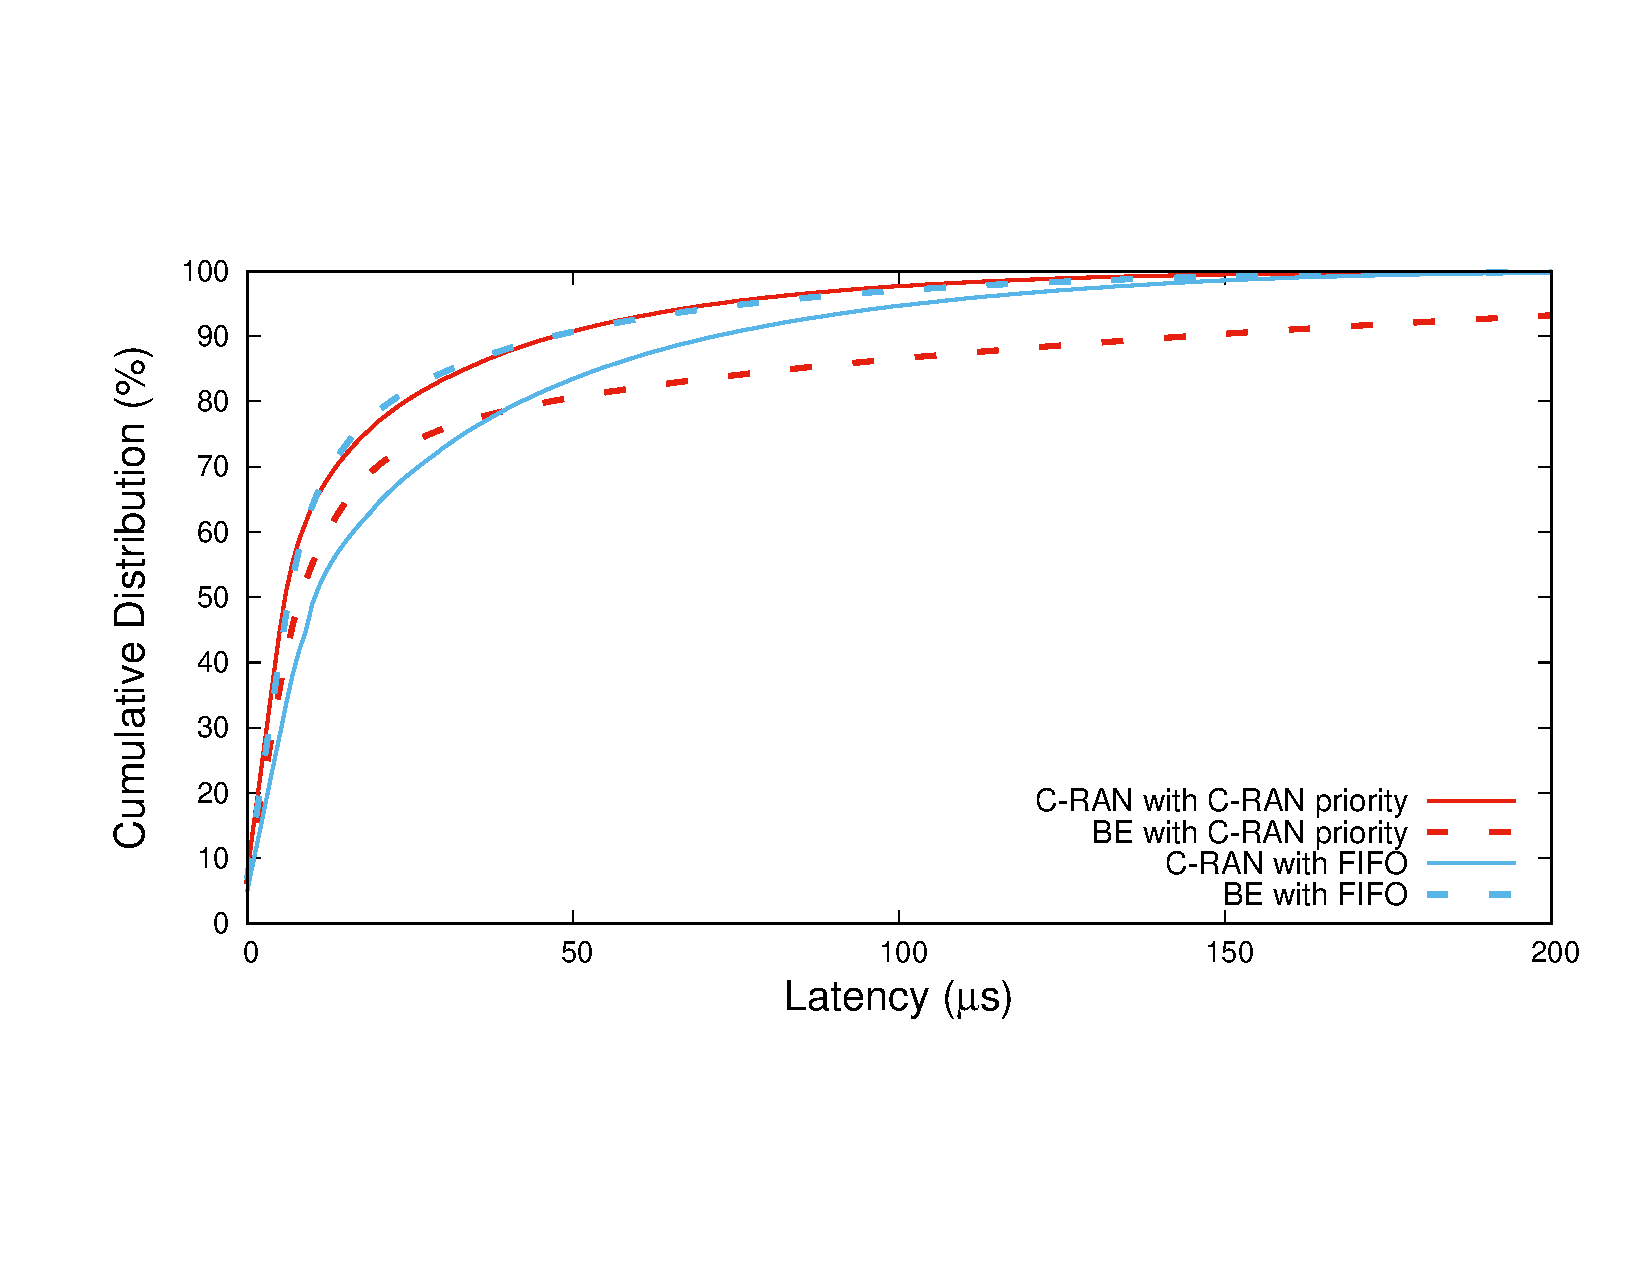
\includegraphics[scale=0.3]{opport.pdf}

     \captionof{figure}{Distribution of latencies for FIFO and C-RAN first}    \label{fig:resultopport}
\end{center} 


\begin{figure}[h]
\begin{minipage}[t]{.46\linewidth}
  
  \scalebox{.55}
  {
  \begin{tabular}{|c|c|}
  \hline
  Bit rate of an electronic interface $R$ & $10$ Gbps \tabularnewline
  \hline
  Optical ring bit rate $F\times R$ & $100$ Gbps \tabularnewline
  \hline
    Acceleration factor $F$ & $10$  \tabularnewline
  \hline
  Container size  $C$ & $100$ kb  \tabularnewline
  \hline
  Unit of time (UoT) $C/(F\times R)$ & $1~\mu$s \tabularnewline
  \hline
  Length traveled during one UoT & $200$ m \tabularnewline
  \hline
    \end{tabular}
  }

\end{minipage} % ne pas sauter de ligne
\begin{minipage}[t]{.46\linewidth}
   \scalebox{.55}
  {
  \begin{tabular}{|c|c|}
  \hline
  Time to go through the cycle $RS$ & $100$ UoT \tabularnewline
  \hline
  Emission time $ET$ & $500$ UoT \tabularnewline
  \hline
   Period $P$ & $1,000$ UoT \tabularnewline
  \hline
  Number of RRH & $5$  \tabularnewline
  \hline
  Number of nodes $k$ & $5$  \tabularnewline
  \hline
   Load induced by C-RAN traffic & $50\%$  \tabularnewline
  \hline
    Load induced by BE traffic & $40\%$  \tabularnewline
  \hline
  \end{tabular}
}
\end{minipage}
  \captionof{table}{Parameters of the N-GREEN architecture}\label{fig:params}
\end{figure}



Unsurprisingly, the latency of the C-RAN traffic is better when we prioritize the C-RAN messages, while the BE traffic is heavily penalized. Furthermore, there is still $10\%$ of the C-RAN traffic with a latency higher than $50 \mu$s, a problem we address in the next section. Remark that the C-RAN and BE traffic latency distribution is not the same with the FIFO method. This comes from the fact that these two sources of traffic are of different nature. With high probability, there are some part of the period which have more 
BE data arrivals (or C-RAN traffic) than average. In both cases, it makes the latency higher during these times. Furthermore, C-RAN traffic is concentrated on half the period, while BE traffic is distributed in all the period.\todo{revoir cette explication}
% However a C-RAN emission from an RRH takes half the period while a BE arrival corresponds to only a few unit of times,
It explains why the C-RAN traffic suffers more from this phenomena.


Remark that, due to the broadcast and select mode, a message coming from any node induces the same load for all the nodes of the ring. Hence the latency of the traffics coming from any RRHs or from the BBU are the same, which may seem couterintuitive knowing that the BBU generates more traffic. This is why in Fig.~\ref{fig:params} we do not ditinguish between uplink C-RAN traffic (RRH to BBU) and downlink  C-RAN traffic (BBU to RRH).

\section{Deterministic approach for zero latency} \label{sec:deterministicalgorithms}
\subsection{Reservation}
Finding good offsets for the C-RAN traffic is a hard problem even for simple topologies and without BE traffic, see~\cite{dominique2018deterministic}. In this section, we give a simple solution to this problem in the N-GREEN optical ring, and we adapt it to minimize the latency of the BE traffic.

Let $u$ be the node to which is attached the RRH $i$, to ensure zero latency for the C-RAN traffic, then the container which arrives at $u$ at time $m_i$ must be free so that the data from the RRH can be sent immediately on the optical ring. 

To avoid latency between the arrival of the data from the RRH and its insertion on the optical ring, 
we allow nodes to \textbf{reserve} a container one round before using it. A container which is reserved cannot be filled by any node except the one which has reserved it (but it may not be free when it is reserved). 
If $u$ reserves a container at time $m_i - RS$, then it is guaranteed that $u$ can fill a free container at time $m_i$ with the data of the RRH $i$.
In the method we now describe, the C-RAN packets never wait in the node: The message sent by the RRH $i$ arrives at its BBU at node $v$ at time $m_i + \omega(u,v)$ and the answer is sent from the BBU at time $m_i + \omega(u,v) +1$.

Recall that an RRH fills a container every $F$ units of time, during a time $ET$. 
Thus if we divide the period $P$ into \textbf{slots} of $F$ consecutive units of time, an RRH needs to fill at most one container each slot. If an RRH emits at time $m_i$, then we say it is at \textbf{position} $m_i + \omega(u,v)\pmod F$.
The position of an RRH corresponds to the position in a slot of the container it has emitted, when it arrives at $u$. 
If an RRH is at position $p$, then by construction, the corresponding $BBU$ is at position $p+1\pmod F$. For now, we do not allow waiting times for C-RAN traffic, hence each RRH uses a container at the same position during all the emission time. 

Given a ring, a set of RRH's, a period and an acceleration factor $F$, the problem we solve here is to find an \textbf{assignment} of values of the offsets $m_i$'s which is \textbf{valid}: two RRHs never use the same container in a period. Moreover we want to preserve the latency of the BE traffic. It means that the time a BE packet waits in the insertion buffer must be minimized. To do so, we must minimize the time a node waits for a free container at any point in the period, by spreading the C-RAN traffic as uniformly as possible over the period. % in order to give the nodes an available container in a minimal average time. 

Figure~\ref{fig:assignment} represents an assignment of two couples of RRH and BBU as the containers going through the node of the BBU during a period. Each slot has a duration of $F$ unit of times, and, since an RRH/BBU emits a packet each $F$ UoT during $ET$ UoT, if we take the granularity of a slot to represent the time, the emission of a BBU/RRH is continuous in our representation, during $ET/F$ slots. A date $t$ in the period corresponds in Figure~\ref{fig:assignment} to the slot $t/F$ and is at position $t \mod F$.


\begin{figure}[h!]
\begin{center}   

      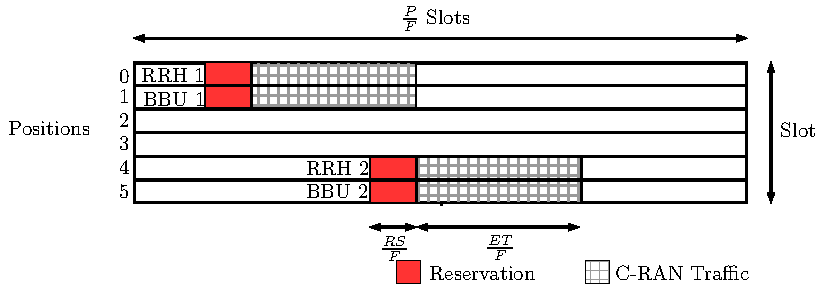
\includegraphics[scale=0.65]{assignment}
     \caption{An assignment with $F = 6$.}\label{fig:assignment}
     
\end{center}
  \end{figure}

 \subsection{Building valid assignment with zero latency}
Remark that two RRHs which are not at the same position never use the same containers. Moreover, if we fix the offsets of the RRHs to even positions so that they do not reserve the same containers, then, because the answers of the BBU are sent without delay in our model, it will fix the offsets of the BBUs to odd positions which do not reserve the same containers. Hence, we need to deal with the RRHs only.
The next proposition gives a simple method to find an assignment.

\begin{prop}
\label{prop:assign}
There is a valid assignment of the offsets $m_1, \dots, m_k$ on the same position if  $k ET + RS \leq P$.
\end{prop}
\begin{proof}
 W.l.o.g we fix $m_1$ to $0$ and all the other offsets will then be chosen at position $0$.  Let $u_1,\dots,u_k$ be the nodes attached to the RRHs $1,\dots,k$. We assume that $u_1,\dots,u_k$ are in the order of the oriented cycle. The last message emitted by the RRH $1$ arrives at $u_2$ at time $ET - 1 + \omega(u_1,u_2)$. Therefore we can fix $m_2 =  ET  + \omega(u_1,u_2)$. In general we can set $m_i = (i-1) \times ET + \omega(u_1,u_i)$ and all RRHs will use different containers at position $0$ during a period. Since $k \times ET + \omega(u_1,u_1) \leq P$ by hypothesis,
 the containers filled by the $k$th RRH are freed before $P$. Hence when the RRH $1$ must emit something at the first unit of time of the second period, there is a free container.
\end{proof}

Remark that reserving free containers make them unusable for BE traffic which is akin to a loss of bandwidth. However, with our choice of emission times of the RRHs in the order of the cycle, most of the container we reserve are used by the data from some RRH. If all containers at some position are used, that is $kET +RS = P$, then there are only $RS$ free containers wasted. In the worst case, less than $2RS$ containers are wasted. 

From Proposition~\ref{prop:assign}, it is easy to derive the maximal number of antennas which can be supported by an optical ring, when using reservation and the same position for an RRH for the whole period.

\begin{corollary}
There is a valid assignment with $ \lfloor\frac{P- RS}{ET}\rfloor \times \frac{F}{2}$ antennas and zero latency.
\end{corollary}
\begin{proof}
Following Prop.~\ref{prop:assign}, the maximal number of antennas for which there is an assignment on the same position is $k = \lfloor\frac{P- RS}{ET}\rfloor $.
In such an assignment, we need a second position to deal with the traffic coming from the BBUs coming back to those k antennas. Since we got  $F$ positions in the slot, the number of antennas supported by the ring is thus equal to $k \times \frac{F}{2}$.
\end{proof}

There are two sources of inefficiency in this method. The first comes from the reservation and cannot be avoided to guarantee the latency of the C-RAN traffic. The second comes from the fact that an RRH must emit at the same position during all the emission time (to guarantee zero latency). In Sec.~\ref{sec:maxant}, we will relax this constraint to maximize the number of antennas supported by the ring, while minimizing the loss of bandwith due to reservation.

We now present an algorithm using reservation as in Prop.\ref{prop:assign} to set the offsets of several RRH at the same position. In the baseline version of the algorithm, we put each RRH in an arbitrary position, for instance one RRH by position. We then propose three ideas to optimize the latency of the BE traffic, by spacing as well as possible the free containers in a period.

\paragraph{Balancing inside the period}

With the parameters of the N-GREEN ring given in Fig.~\ref{fig:params} ($ET = \frac{P}{2}$, $F = 10$ and $n = 5$), there are no unused position. Any assignment has exactly one  BBU or RRH at each position. If all the RRHs start to emit at the first slot, then during $ET$ there will be no free container anywhere on the ring, inducing a huge latency for the BE traffic. 
To mitigate this problem, in a period, the time with free containers in each position must be uniformly distributed over the period as shown in Fig.~\ref{fig:periodbal}.
\begin{figure}[h!]
\begin{center}   

      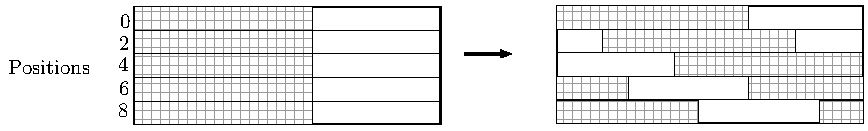
\includegraphics[scale=0.55]{repart2}
     \caption{Balancing inside the period.}\label{fig:periodbal}
     
\end{center}
  \end{figure}  
  

  
\paragraph{Compacting positions}

For each position which is used by some RRH, and during each period, $RS$ containers are reserved before starting to emit some C-RAN traffic, while they can be free. Hence, it decreases the maximal load the system can handle.
Therefore to not waste bandwidth, it is relevant to put as many RRHs as possible on the same position as in Fig.~\ref{fig:packing}. Indeed, for any position which is not used at all, $RS$ containers need not to be reserved. This strategy is also good for the latency of the BE traffic. If a position is unused, then there is always a container free of C-RAN traffic each $F$ unit of times. 
\begin{figure}[h!]
\begin{center}   

      \includegraphics[scale=0.5]{repart0}
     \caption{Compacting positions.}\label{fig:packing}
     
\end{center}
  \end{figure}
  

\paragraph{Balancing used positions}

The free positions can be distributed uniformly over a slot, to minimize the time to wait before a node 
has access to a free container, as shown in Fig.~\ref{fig:slotbal}. To do so, compute the number of needed positions $x = \lceil k\times \frac{ET}{P - RS}\rceil$, with k the number of antennas. Then, set the $x$ used positions in the following way: $\lfloor\frac{F}{x}\rfloor -1 $ free positions are set between each used positions. If $\frac{F}{x}$ has a reminder $r$, then we set the $r$ free remaining positions uniformly over the interval in the same way and so on until there are no more free position. It is a small optimization, since it decreases the latency by at most $F/2$.

\begin{figure}[h!]
\begin{center}   

      \includegraphics[scale=0.55]{repart1}
     \caption{Balancing used positions.}\label{fig:slotbal}
     
\end{center}
  \end{figure}

  \paragraph{Experimental evaluation}

  In order to understand the contribution of the three ideas presented in the previous subsection,
   we present the cumulative distribution of the latency of the BE traffic latency.
   
Fig.~\ref{fig:periodonly} shows the performance of balancing the C-RAN traffic inside the period against a baseline version in which all the RRH begin to emit at the same slot. We keep the same parameters as in the previous experiment, described in Table~\ref{fig:params}. The BE traffic latency is highly decreased when we balance the C-RAN traffic inside the period.

 Since the N-GREEN parameters does not allow us to put several RRH at the same position, we changed the emission time to $ET = 200$ To keep the load around $90\%$ as in the experiment of Fig.~\ref{fig:resultopport}, we set $n = 12$. This is not out of context since the exact split of the C-RAN (the degree of centralization of the computation units in the cloud) is not fully determined yet~\cite{mobile2011c}. With these parameters, the loss of bandwidth due to reservation is at most $6\%$

As show in Fig.\ref{fig:algocmp}, the performance when we do no compacting positions is really bad, even worst than the methods using an insertion buffer. It is explained by the parameters of the N-GREEN ring: all positions are used and thus, there are no free containers available to BE traffic during $ET+RS$ units of time. When compacting the RRHs on a minimal number of positions, the latency decreases dramatically and becomes much better than in the previous methods. The optimizations of balancing used positions brings almost no benefit as expected: The average (respectively maximum) latency for BE traffic is $4.43\mu$s (resp. $44\mu$s) instead of $4.76\mu$s (resp. $48\mu$s) with compacting position only. Also, the balancing over a period improves the latency marginally when compacting positions is possible. 


In Fig.~\ref{fig:optimres}, we compare the cumulative distribution of the latency of the BE traffic using the FIFO rule or the reservation algorithm proposed here. 

  The performance of the reservation algorithm is excellent, since the C-RAN traffic has {\bf zero latency} and the BE traffic has a \textbf{better latency} with reservation than with the FIFO rule. It is due to the balancing of the load of the C-RAN traffic over the period, that guarantee a more regular bandwidth for the BE traffic.
  


\begin{figure}[h!]
\begin{center}   

      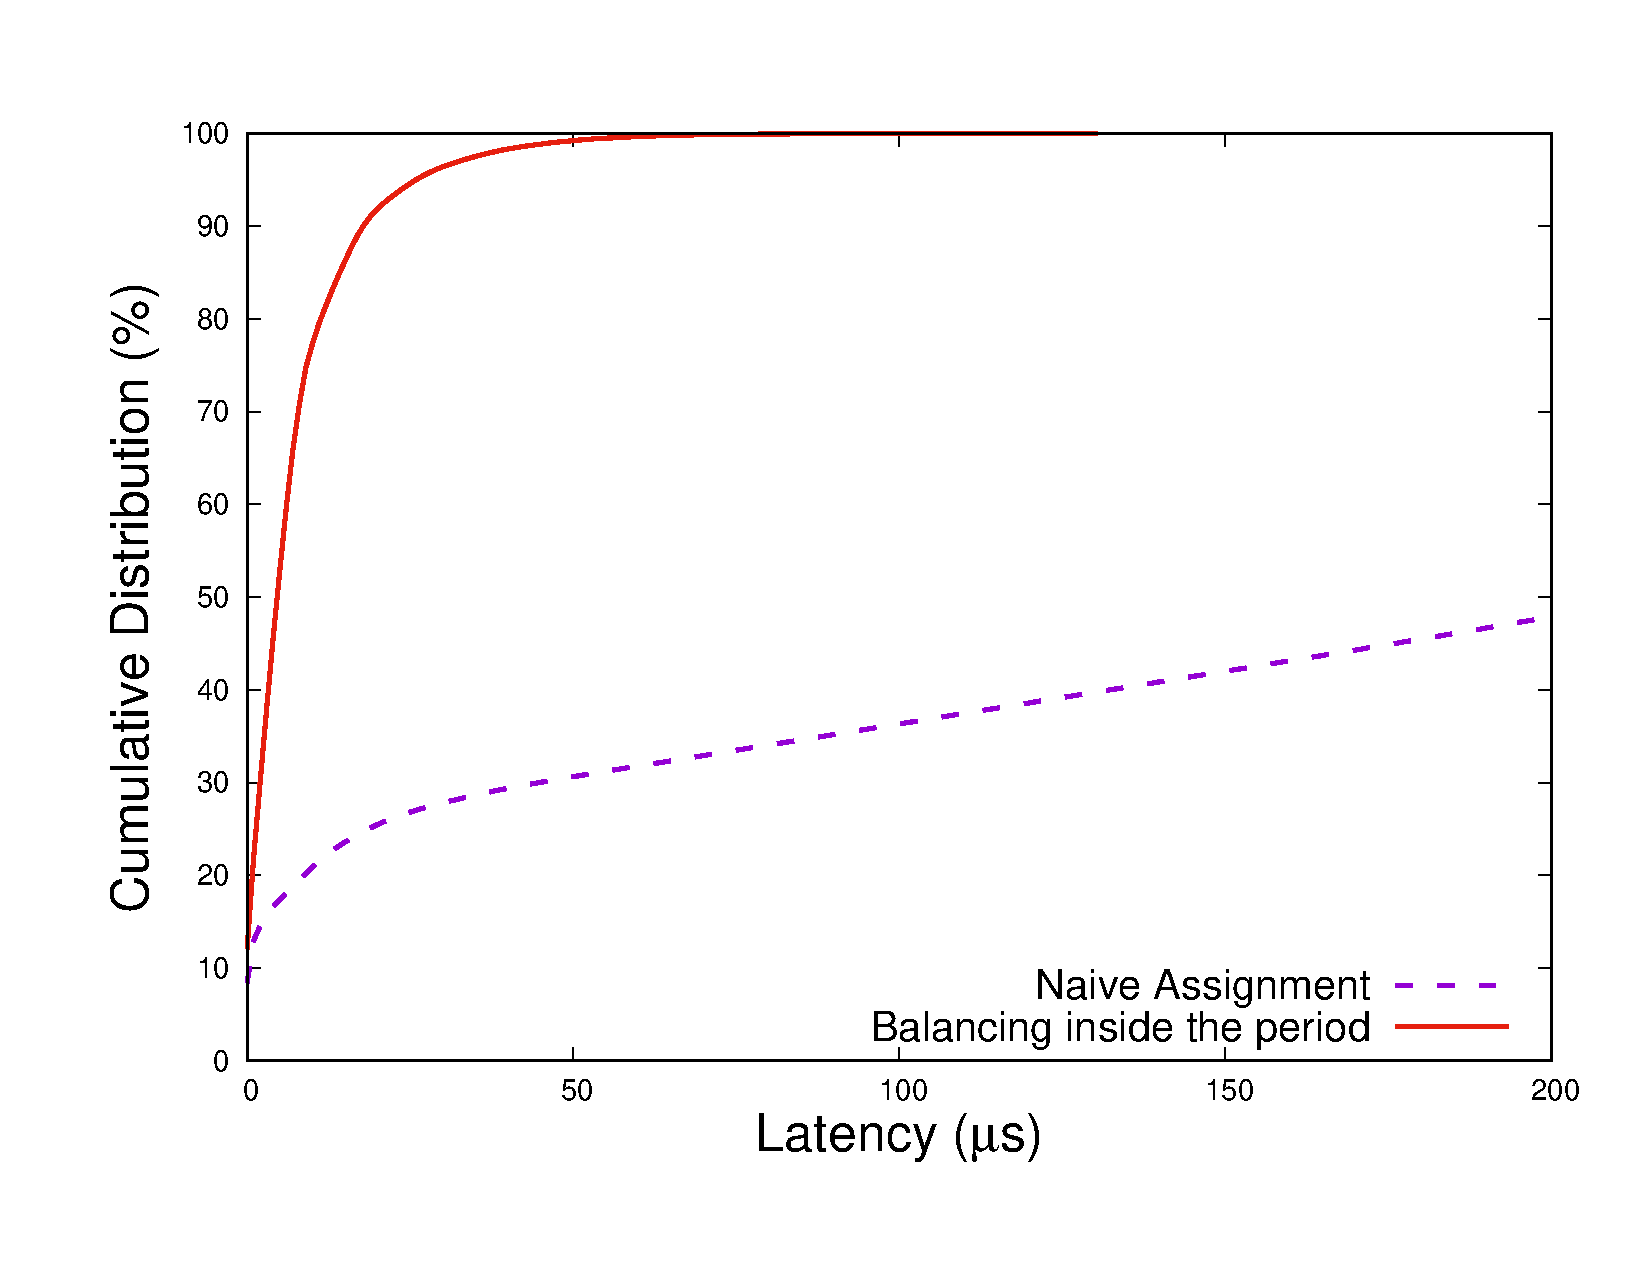
\includegraphics[scale=0.25]{periodonly}
     \caption{Impact of balancing the inside the period on the BE traffic latency.}\label{fig:periodonly}
     
\end{center}
  \end{figure}
  
\begin{figure}[h!]
\begin{center}   

      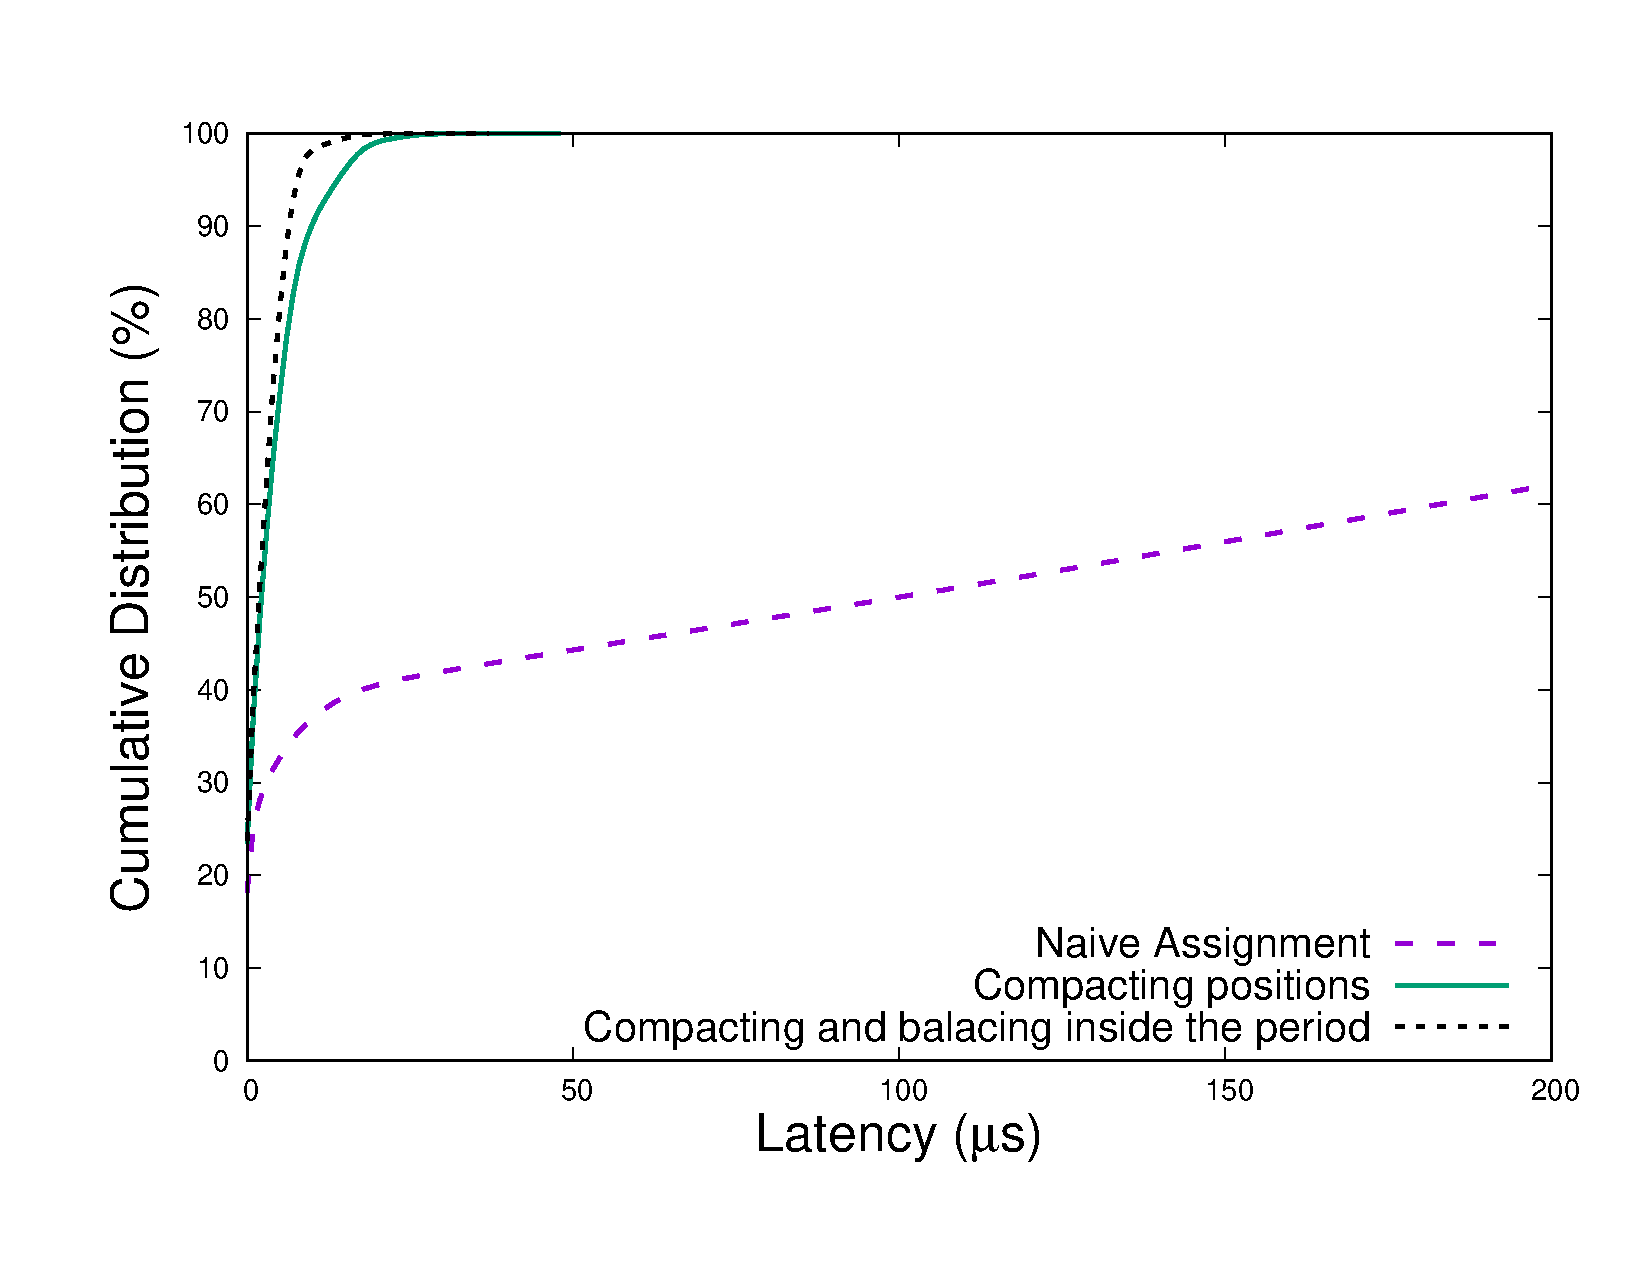
\includegraphics[scale=0.25]{repart1res}
     \caption{Impact of compacting position on the BE traffic latency.}   \label{fig:algocmp}
\end{center}
  \end{figure}
  
  
  
  \begin{figure}[h!]
\begin{center}   

     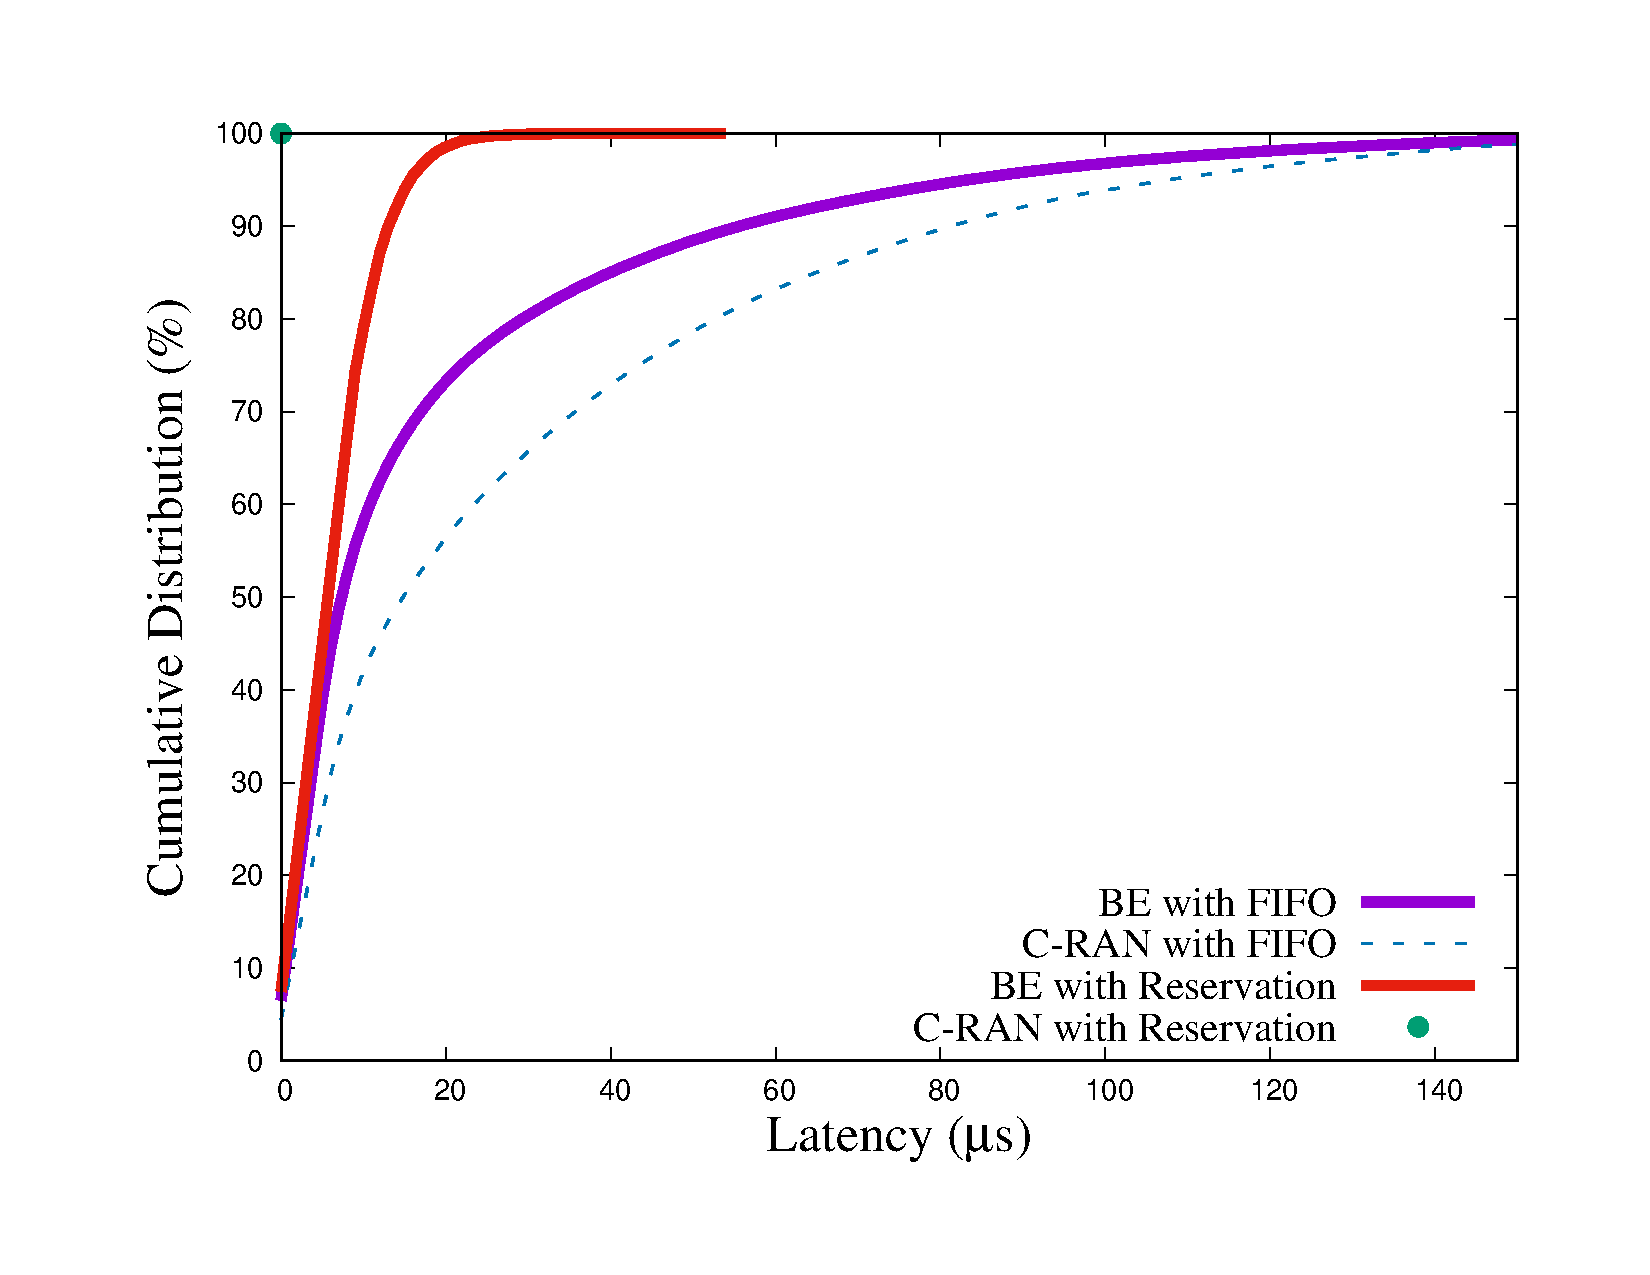
\includegraphics[scale=0.25]{optim.pdf}
     \caption{Impact of the deterministic method on the traffics.}   \label{fig:optimres}

\end{center}
  \end{figure}
  
\subsection{Valid assignment with small C-RAN latency}
\label{sec:maxant}

The previous approach limits the number of antennas supported by the ring when $P-RS \mod ET \neq 0$, which is the case with N-GREEN parameters. In order to maximize the number of supported antennas (and to minimize the reserved containers), we now \emph{allow the data from an RRH to use different positions}. 

\todo{dire le tradoff -> en échange de plus d'antennes et d'une meilleure latence BE on a une 
petite perte sur les C-Rans et une augmentation raisonnable de complexité (buffering pour les CRAN).}


\paragraph{Filling positions}

In order to support as much antennas as possible on the ring, we use \emph{all} containers in a given position, improving on the compacting position heuristic. 

\begin{prop}
 There is a valid assignment for $k$ antennas when $k \leq \lfloor \frac{P- RS}{ET} \times \frac{F}{2}\rfloor$.
\end{prop}


To do so we assign the antennas to the first position which is not full. When less than $ET$ free containers remain in this position (let us call $x$ this number of free containers), then the $x$ first containers of an antenna are assigned to this position, and the $ET - x$ last containers of this antennas are assigned to the next position. Fig.~\ref{fig:split} illustrates this manner to find an assignment with a maximal number of antennas. 


\begin{figure}[h!]
\begin{center}   

      \includegraphics[scale=0.8]{split}
     \caption{Assignment with $9$ antennas with the N-GREEN parameters.}   \label{fig:split}
\end{center}
  \end{figure}
  
  This reservation algorithm naturally apply the compacting position of the previous subsection. Also, there is no balancing into the period to do because all the used position (except the last) are full. The only possible optimisation for the best effort traffic would be to balance the used positions, but, it would add some additional latency on the packet which are already assigned with $2$ unit of time of delay.
  Since the N-GREEN parameters only allows to do balancing into the period of the previous section, we want to compare the impact on the best effort traffic of fulfilling positions against balancing into the period and FIFO rule. 
Fig.~\ref{fig:splitres} represent the cumulative distribution of the best effort traffic with those three methods, and with the N-GREEN parameters.


\begin{figure}[h!]
\begin{center}   

      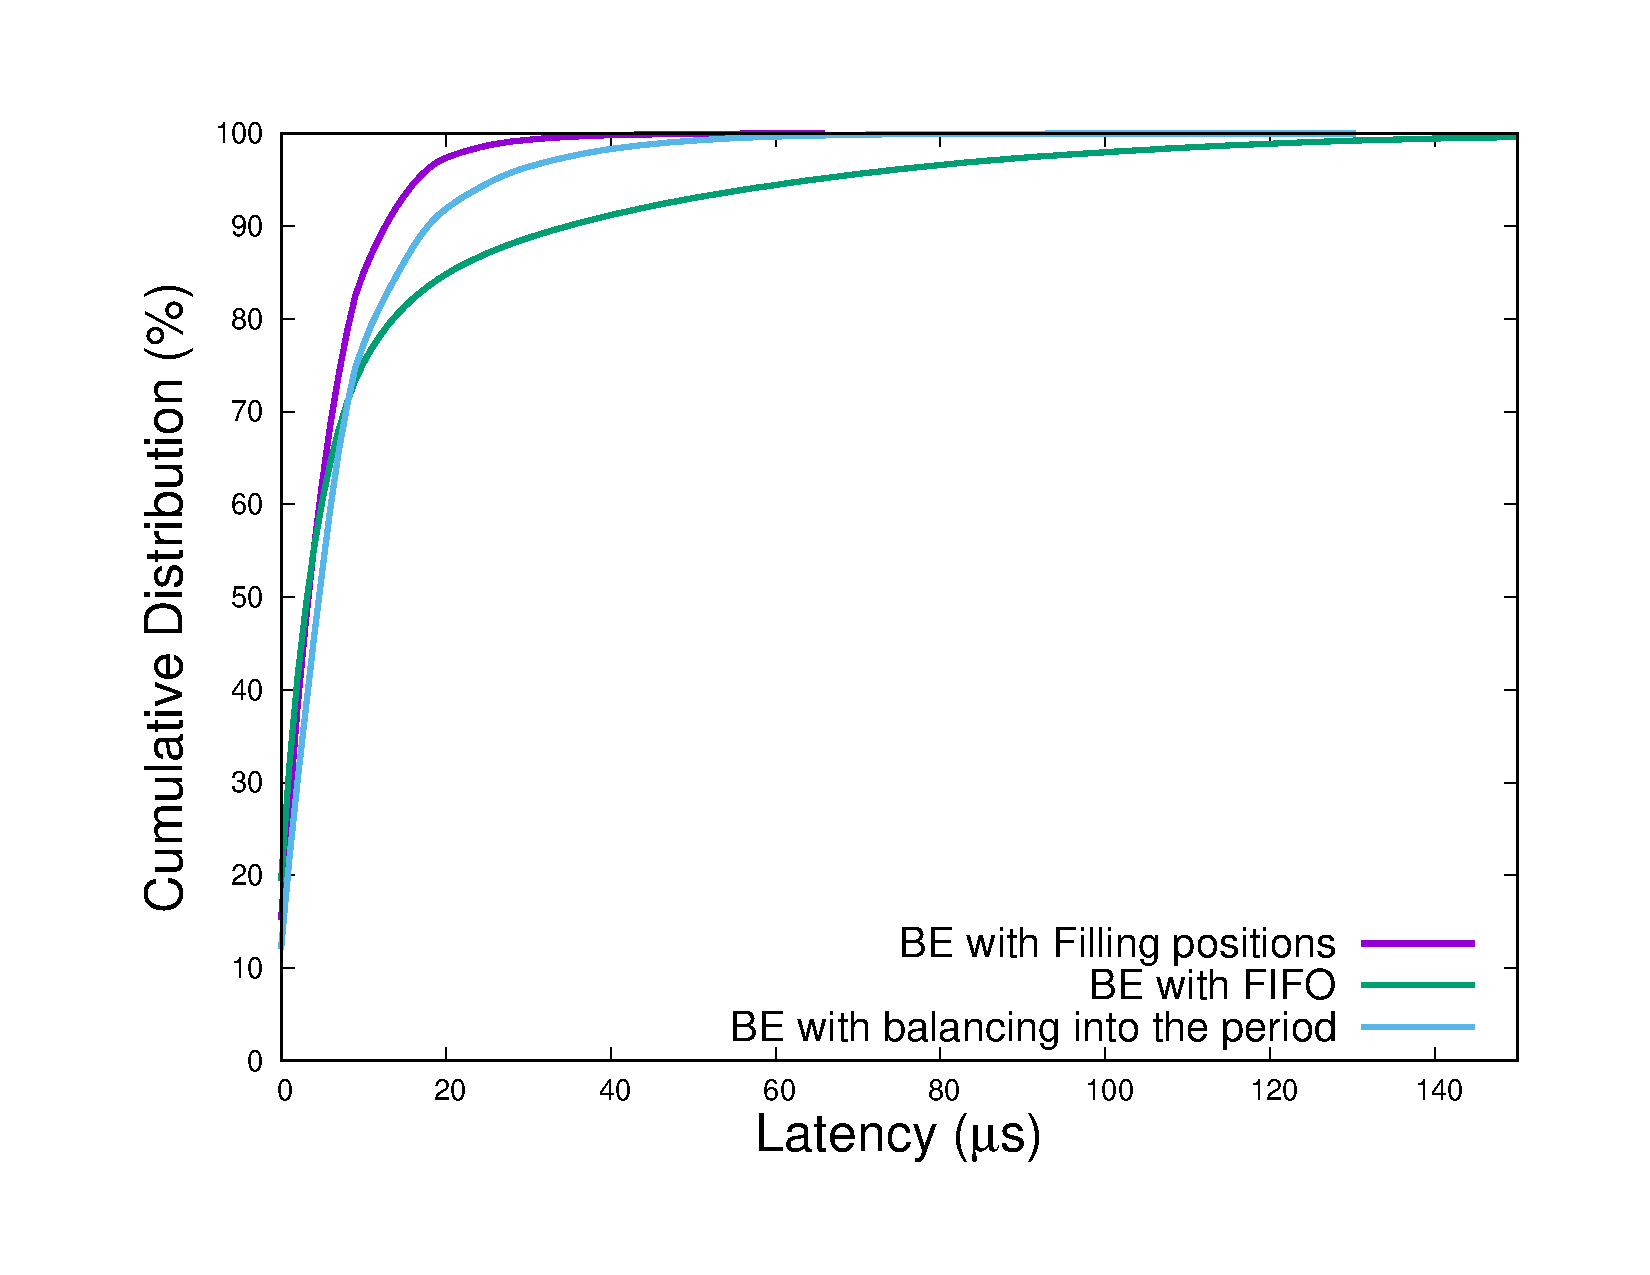
\includegraphics[scale=0.25]{splitres}
     \caption{Impact of fulfilling positions on BE traffic.}   \label{fig:splitres}
\end{center}
  \end{figure}
  
  \section*{Conclusion}
  
  
  \bibliographystyle{ieeetr}
\bibliography{src}

\end{document}
